\documentclass[a4paper, 12pt]{article}

\usepackage[T1]{fontenc}
\usepackage[utf8]{inputenc}
\usepackage[english]{babel}  % ngerman for German
\usepackage{lmodern}  % nicer font
\usepackage{geometry}
\geometry{%
	left   = 2.5cm,
	right  = 2.5cm,
	top    = 3cm,
	bottom = 3cm
}

\usepackage{textcomp}
\usepackage{gensymb}
\usepackage{amsmath,amssymb,amsfonts}
\usepackage{nicefrac}  % nicer inline fractions
\usepackage{tensor}  % allows fancy indices
\usepackage{siunitx}  % easy handling of value + unit (e.g. \SI{10}{\pF})
% \sisetup{}  % configure siunitx (e.g. locale = DE)
\sisetup{output-complex-root=\ensuremath{\mathrm{j}}, complex-root-position = before-number} % configures SI format 10 + j5 for complex numbers (instead of 10 + 5i)

\usepackage{listings}  % code listings
\usepackage{verbatim}  % inline code (\verb||)
\usepackage{enumerate}
\usepackage[shortlabels]{enumitem}  % simple format for enumerations (e.g. 
\usepackage{booktabs}  % nicer tables (e.g. \toprule)
\usepackage{subcaption}  % captions for subplots
\usepackage[european, siunitx, RPvoltages]{circuitikz}  % draw circuit diagrams

\setlist[itemize]{label=\rule[0.5ex]{0.6ex}{0.6ex}} % black squares for itemize

\usepackage{pstool}  %% Tex fonts in EPS files
\usepackage{graphicx}
\graphicspath{{./figures/}}

\setlength {\marginparwidth }{2cm}  % fixes issue with todonotes
\usepackage{todonotes}
\usepackage{etoolbox} % Needed for AtBeginEnvironment command (appendix handling)
\usepackage{appendix} % Appendices environment

\usepackage{csquotes} % removes biber warning
\usepackage[  % ieee style citations (e.g. [1])
	backend     = biber,
	maxbibnames = 99,
	autocite    = footnote,
	style	    = ieee,
	citestyle   = numeric-comp,
	doi=false, isbn=false
]{biblatex}
\addbibresource{bibliography/bibliography.bib}

\usepackage[nobiblatex]{xurl}  % line breaks in URLs
% last imports
\usepackage[bookmarksopen,colorlinks,citecolor=black,linkcolor=black, urlcolor = black]{hyperref}

% after hyperref! 
\usepackage[noabbrev, nameinlink]{cleveref} 
% e.g. \cref{label} or \Cref(label) for capital letter
% configure cleveref not to use brackets around equation references
\creflabelformat{equation}{#2\textup{#1}#3} % Equation references without parentheses
\AtBeginEnvironment{appendices}{\crefalias{section}{appendix}} % Appendix referencing (for cref "Appendix A" instead of "Section A")


% add missing hyphenations
\hyphenation{im-ple-men-ta-tions}

\title{384.180 SoC Advanced Course\\
	   Integration of an Encryption Accelerator
	   into an Open-Source Low-Power Microcontroller}
\author{
  Severin Jäger, 01613004
}
\date{\today}


\begin{document}

\maketitle
\tableofcontents
\pagebreak

\section{Introduction} \label{sec:intro}

Extreme edge devices are increasingly expected to perform signal processing workloads. Sensor signals are frequently processed directly in the sensor node before being transmitted for further analysis. Examples include simple machine learning algorithms detecting relevant sequences or events in a sensor signal. However, such edge devices are usually battery-powered and designed for a long lifetime, thus the energy consumption is highly constrained. So, applications have to be designed with energy efficiency in mind. This is also a main factor when partitioning between hardware and software.

One major academic project focussing on energy-efficient processor and system design is the PULP platform~\cite{pulp} by ETH Zurich and University of Bologna. Over the last years, they developed several processor cores as well as peripherals and full systems on chips (SoCs). Utilising the open source instruction set architecture RISC-V, the RTL code of the IP cores developed within this project is available publicly with a permissive license.

In certain applications including biomedical devices, video surveillance, or home automation, traditional requirements are complemented by a need for confidentiality. Thus, standard cryptographic algorithms have to be executed on the edge hardware. Unfortunately, processing these algorithms in software is relatively complex and consumes significant memory, time, and thus energy. These issues might however be alleviated by offloading the computation to a dedicated cryptographic accelerator. The scope of this project is integrating and open-source hardware accelerator into the PULPissimo SoC~\cite{Schiavone2018} and comparing it to a pure software solution. Additionally, an FPGA demonstration and a partial ASIC synthesis are part of this project.

\section{Background} \label{sec:background}

\subsection{PULPissimo}

PULPissimo is a microcontroller and as such one of the smallest platforms within the PULP ecosystem. It comes with a single RISC-V core, memory, a DMA controller, and a full set of peripherals controlled via a bus. Furthermore, it allows the convenient integration of a so-called hardware processing engine (HWPE) which directly operates on the memory. The SoC architecture is depicted in \cref{pulpissimo-arch}.

\begin{figure}
	\centering
	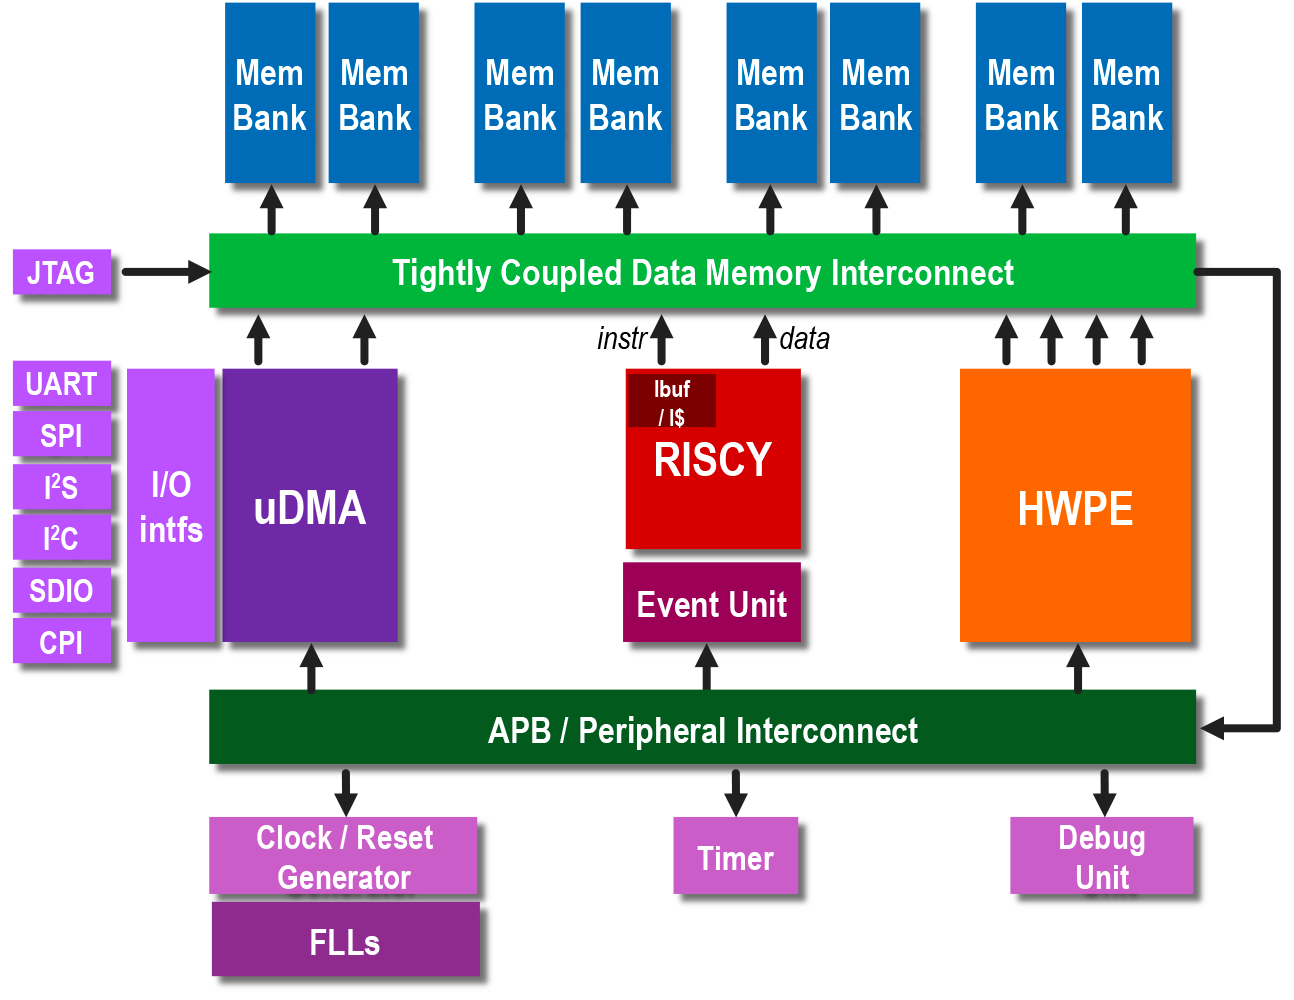
\includegraphics[width=0.6\textwidth]{pulpissimo_arch.png}
	\label{pulpissimo-arch}
	\caption{Architecture of the PULPissimo SoC \cite{pulpissimo}}
\end{figure}

The design is mainly targeting ASIC technology and focussed on maximum energy efficiency. In a \SI{22}{nm} FDX technology, an energy efficiency of \SI{433}{MOPS/mW} has been shown~\cite{Schiavone2018}. The full System Verilog RTL code including scripts for simulation and FPGA evaluation is available on GitHub~\cite{pulpissimo}.

\subsubsection*{Hardware Processing Engine (HWPE)}

The PULP hardware processing engine is a quite unique hardware accelerator. As depicted in \Cref{hwpe-arch}, it consists of a data interface, a control interface and the data path. In contrast to most accelerators in literature it neither uses a dedicated accelerator interface in the CPU nor direct memory access (DMA) to get the data to the processing units. Instead, it shares the so-called tightly coupled memory (which somehow corresponds to an L2 cache) with the processor core. The control interface is connected to the peripheral bus and is thus seen as a memory-mapped peripheral by the CPU. It provides configuration registers which can be written by the processor.

\begin{figure}
	\centering
	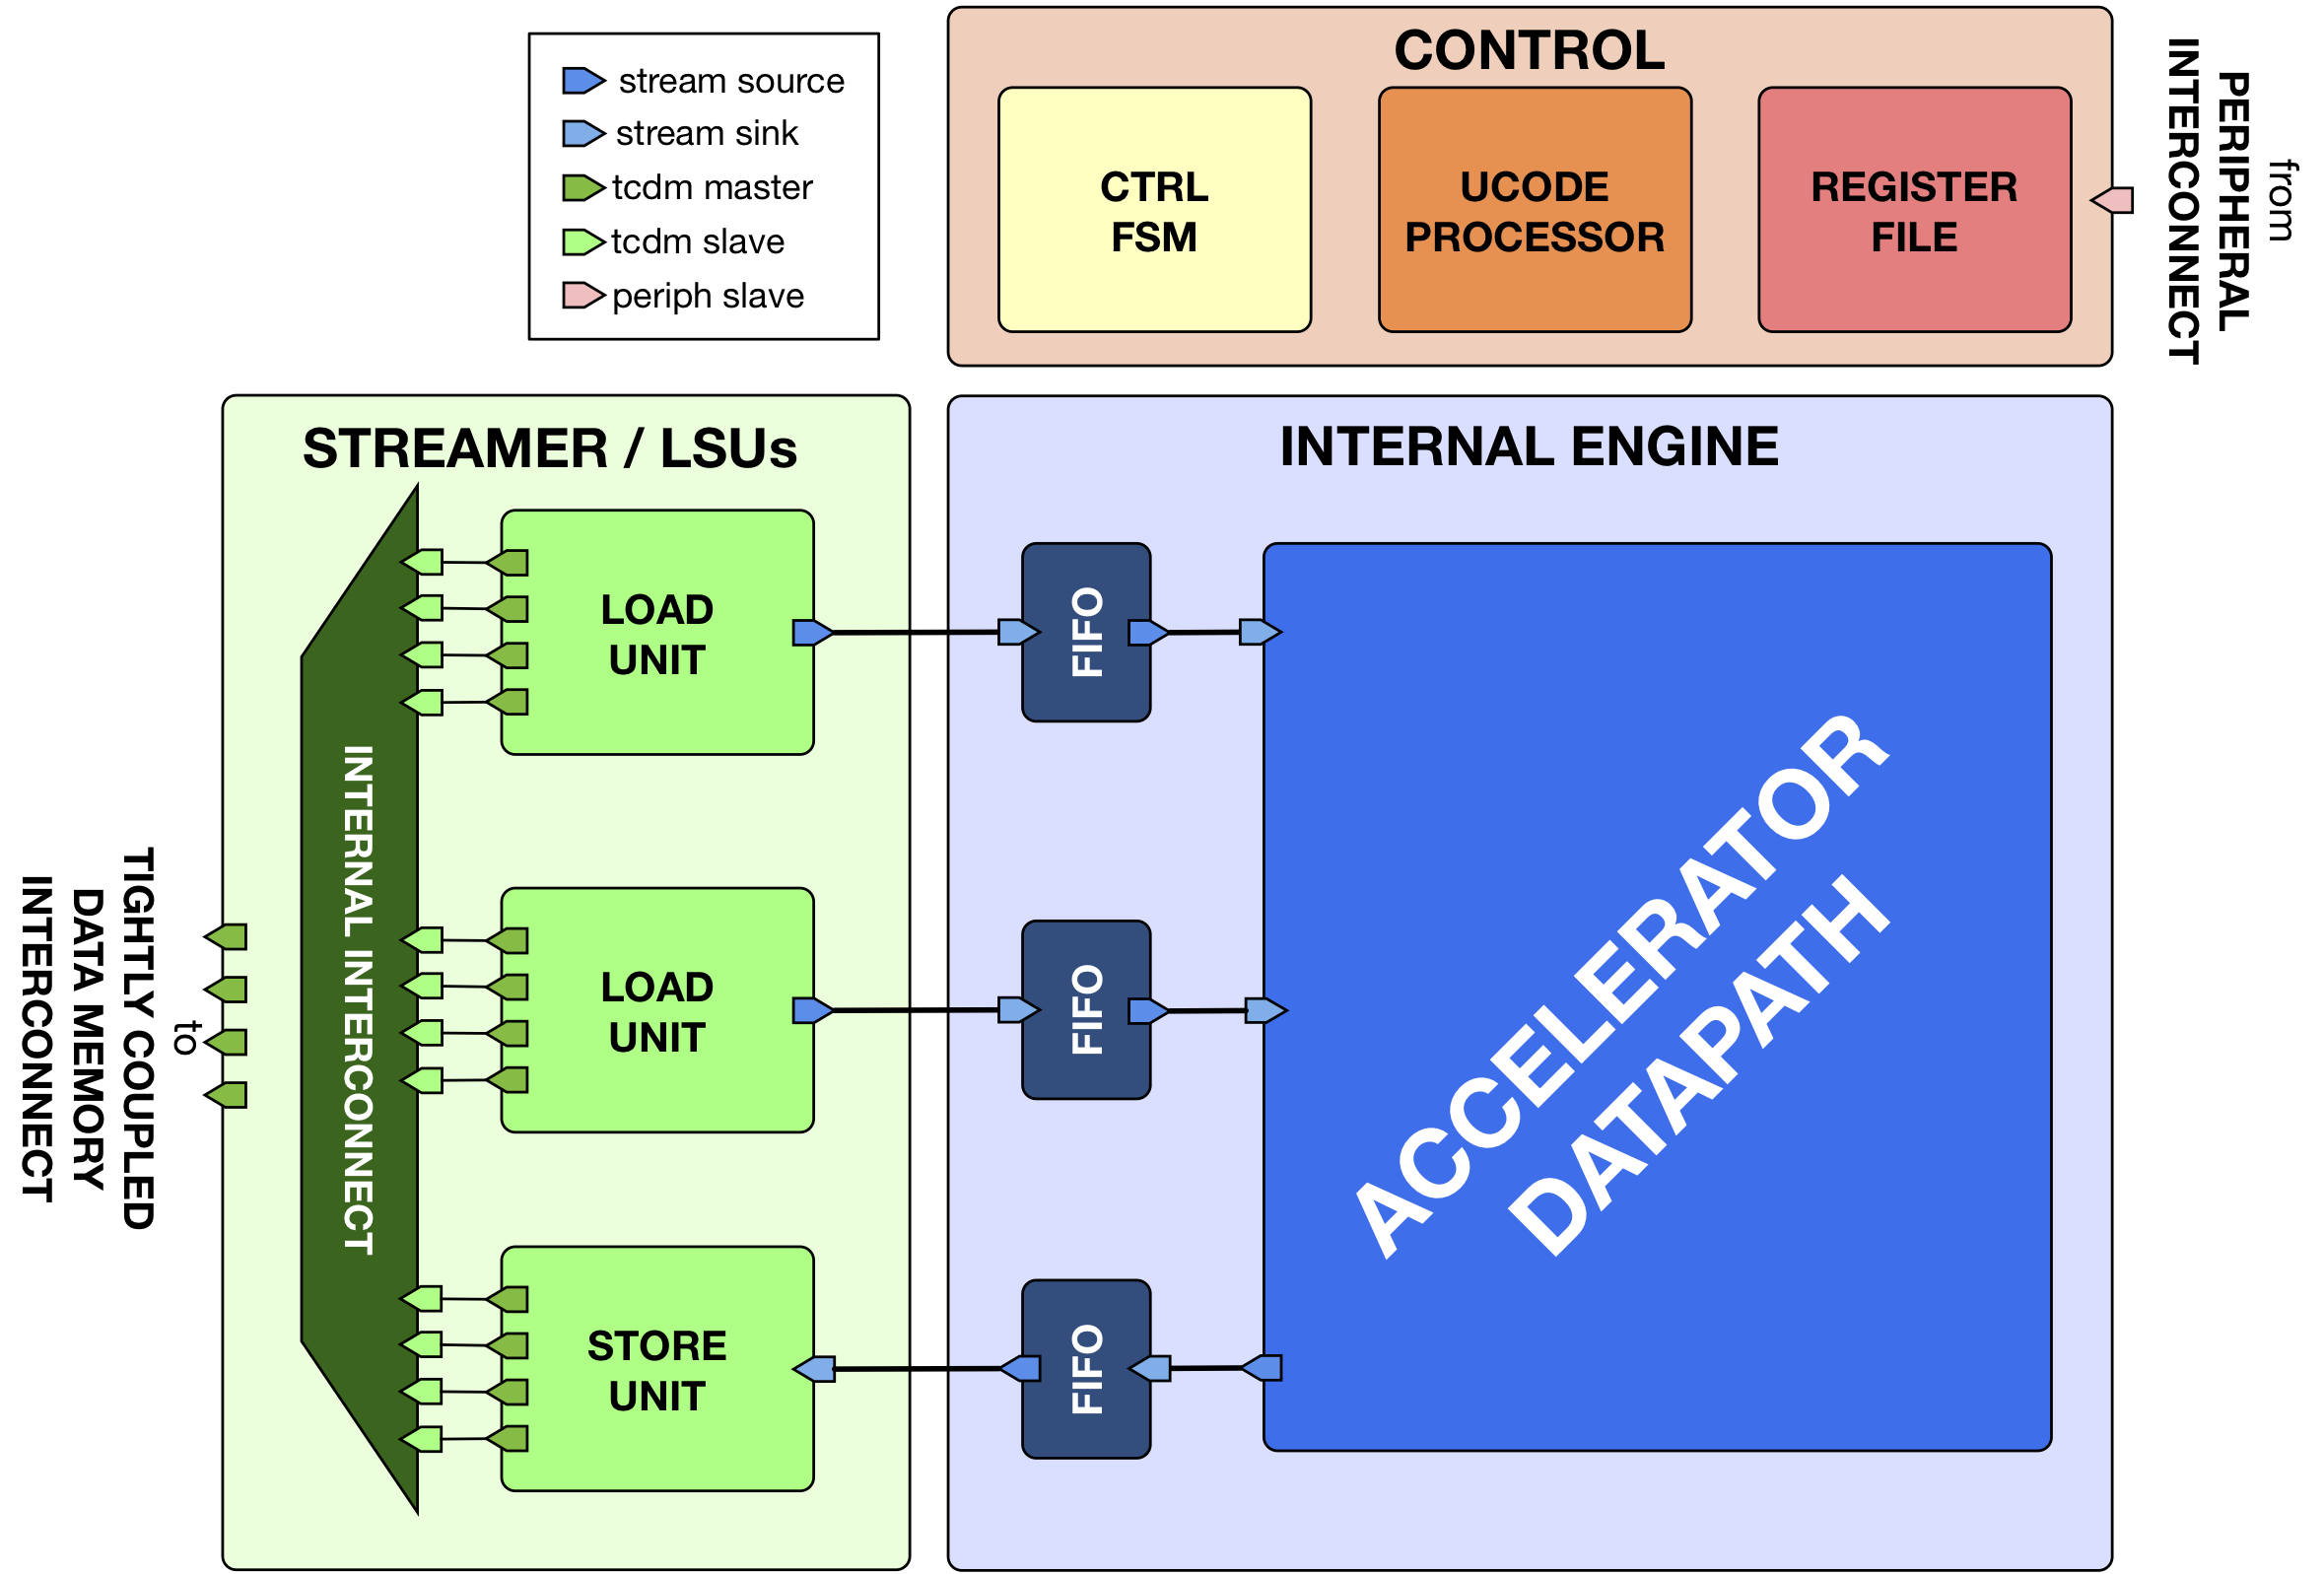
\includegraphics[width=0.65\textwidth]{hwpe.png}
	\label{hwpe-arch}
	\caption{Architecture of a PULP Hardware Processing Engine \cite{hwpe}}
\end{figure}

A typical HWPE operation works as follows. Firstly, the relevant data has to be placed in the shared memory. Then, the CPU sets all relevant configuration data (e.g. pointers of source and destination in shared memory, data size, HWPE configuration) via the HWPE´s control interface. Once a HWPE operation is started, it operates fully autonomous and the CPU can perform other computations. After completion, the HWPE trigger and event which can be polled in the CPU or raise an interrupt. The event indicates that the output data is written to the shared memory.

HWPEs are not limited to PULPissimo, but can also be integrated into more powerful SoCs within the PULP project including multicore systems and HPC clusters. Thus, the effort of designing an HWPE can be reused easily. Furthermore, a template HWPE implementing a multiply-accumulate (MAC) engine is available~\cite{hwpe-mac}. This template features a relatively simple data path, but a powerful control interface including a microcode processor and a finite state machine as well as three 32 bit inputs and one 32 bit output. The template is intended as starting point for new HWPEs and alleviates the burden of the developer to write a device driver and to handle the memory access. The work in this project is based on this template.

\subsection{AES Hardware}

The advanced encryption standard (AES) defines a set of block cipher algorithms which are also known under their original Dutch name Rijndael. It works on 128-bit words and uses either 128, 192, or 256-bit keys. The algorithm was designed for straightforward hardware implementation and is one of the most frequently used block ciphers.

In general AES operates in rounds (10 for 128-bit keys) which consist of different mathematical steps. Hardware implementations might implement these operations once and compute the round results sequentially or pipeline them to some extent. The most powerful implementation consists of 10 parallel round hardware blocks which are pipelined.

Thus, several hardware implementation of the AES algorithms are available. As this project uses open-source System Verilog RTL code, only permissively-licensed open-source Verilog implementations were considered. \Cref{tab:aes_cores} compares the three IP cores considered. An edge device requires only encryption capabilities to transfer sensor data in a secure way. Also due to size and energy limitations, only AES with 128 bit keys was considered.

\begin{table}[h]
    \centering
    \begin{tabular}{c|c c c}
        \toprule
        Core &  \verb|tiny_aes|~\cite{tiny-aes} & \verb|aes_128|~\cite{aes-128} & \verb|secworks_aes|~\cite{secworks-aes}  \\
        \midrule
        Cycles/Op &  1 & 12 & 4\\
        Latency (cylces) & 21 & 12 & 14\\
        LUTs & 4588 & 487 & 3327 \\
        Registers & 4474 & 402 & 2990 \\
        BRAM Tiles & 68 & 5 & 0 \\
        Max. Frequency [MHz] & 375.9 & 180.5 & 124.8 \\
        Decryption & no & yes  & yes \\
        256 bit keys & no & no & yes\\
        \bottomrule
    \end{tabular}
	\label{tab:aes_cores}
	\caption{Comparison of selected open-source AES IP cores. Resource consumption and clock frequency were obtained with Vivado 2020.2 synthesising for a Nexys~4~DDR evaluation board.}
\end{table}

Clearly, the \verb|tiny_aes| core provides the best performance. It is fully pipelined and thus has the highest throughput and the shortest critical path. In contrast, \verb|aes_128| is a highly minimal design that reuses the stages of the AES algorithm to minimise hardware resources. In between, the \verb|secworks_aes| core finds a trade-off and optionally offers several features that are not required for this project (decryption or larger keys). Given the energy constraints and the most likely relatively low number of transmissions required, the \verb|aes_128| IP core was selected to be integrated into PULPissimo as HWPE.

\section{Baseline Implementation} \label{sec:implementation}

A first step towards integrating the \verb|aes_128| core into PULPissimo was already taken in a prior course. This report mainly focusses on the new contributions. Still, a wrap-up of the prior work is given in this section for easier understanding.

\subsection{Setup} \label{sec:implementation:setup}

As PULPissimo is written in System Verilog and the scripts require either Mentor Questasim or Cadence Xcelium, an ICT EDA server was used to run the Mentor toolchain. This required working on the server file system and mounting the relevant directories via ssh on the local machine as all required dependencies for compilation are installed there. As the PULPissimo scripts make use of environment variables frequently, doing so required several scripts, some of the are located in the \verb|scripts| directory in this repository.

\subsection{Reference Software}

To have a reasonable baseline, a software implementation of the AES algorithm was required. Due to its small code size which perfectly fits microcontroller environments, the Tiny AES in C~\cite{tiny-aes-c} implementation was chosen. It easily compiles for PULPissimo with the PULP SDK and requires only around \SI{2}{kiB} of memory. The software library offers several encryption modes and key sizes. However, for the first version only electronic code book (ECB) encryption capability with 128 bit keys was used. 

\subsection{Hardware Processing Engine}

The design of the AES HWPE supports only 128-bit ECB encryption and is based on the PULP MAC engine template~\cite{hwpe-mac}. It contains the AES IP core as well as units converting the 32-bit memory words to 128-bit AES keys and words (byte\_stackers and byte\_unstacker). The resulting AES HWPE is depicted in \Cref{hwpe-aes}. The input and output streamers are controlled by the FSM in the control block which uses the registers written by the CPU beforehand. All data path units use a simple ready/valid handshake to allow both forward and backward dependencies, e.g. if the AES unit is busy of no new data is provided by the input streamers yet.

\begin{figure} [h]
	\centering
	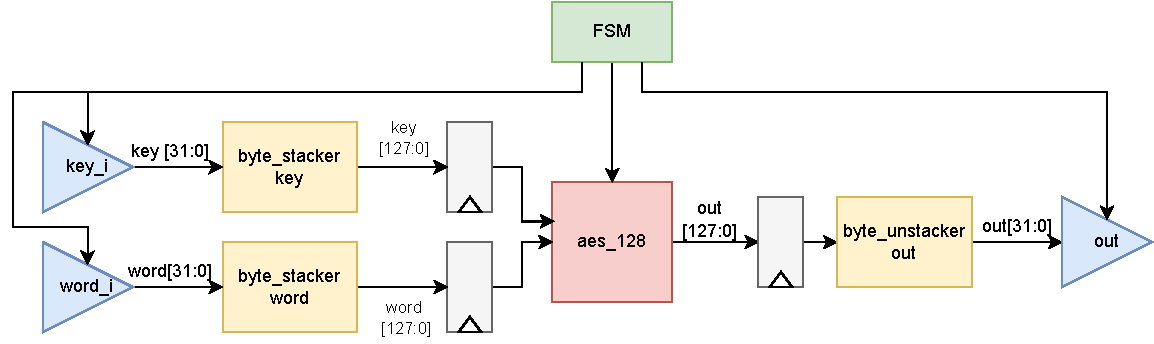
\includegraphics[width=0.95\textwidth]{hwpe_aes.pdf}
	\label{hwpe-aes}
	\caption{Block diagram of the implemented AES HWPE}
\end{figure}

\section{Improved AES Engine} \label{sec:improvements}

The work described from here on was conducted during the SoC Advanced course. Firstly, the AES engine has been improved and demonstrated on an FPGA. Additionally, an ASIC synthesis flow was performed, this is described in \Cref{sec:asic}.

\subsection{Register Reduction}

In a first step, the pipelining registers depicted in \Cref{hwpe-aes} were removed. They added area as well as increased the latency without providing any value to the timing behaviour as both the byte\_stacker modules and the AES IP core already provide pipelining registers at their outputs.

\subsection{Cipher Block Chaining}

As the electronic code book encryption mode produces identical output values for identical input blocks, it lacks the so-called diffusion property and is thus not considered safe. Therefore, the AES core was extended to support the cipher block chaining (CBC) mode of operation. Here, the plain test is XORed with the last ciphertext to produce different outputs for identical inputs, s. \Cref{fig:cbc}.

\begin{figure} [h]
	\centering
	
\includegraphics[width=0.65\textwidth]{cbc.png}
	\label{fig:cbc}
	\caption{Cipher block chaining mode of operation \cite{wiki_cbc}}
\end{figure}

Adding CBC support to the AES HWPE requires only small modifications. Firstly, a register storing the last ciphertext is required. Then, a 128-bit xor block has to be added. The result is shown in \Cref{hwpe-aes-update}. As the pipeline features a ready-valid handshake system which is not depicted, some additional handshake signals are required to ensure that each ciphertext is used exaclty once. The reset value of the ciphertext register is the initialisation vector (IV), which is in the current implementation hardwired. In principle, it is possible to make the IV configurable via the peripheral bus interface. A further conceivable improvement is a configuration bit that allows switching between ECB and CBC.

\begin{figure} [h]
	\centering
	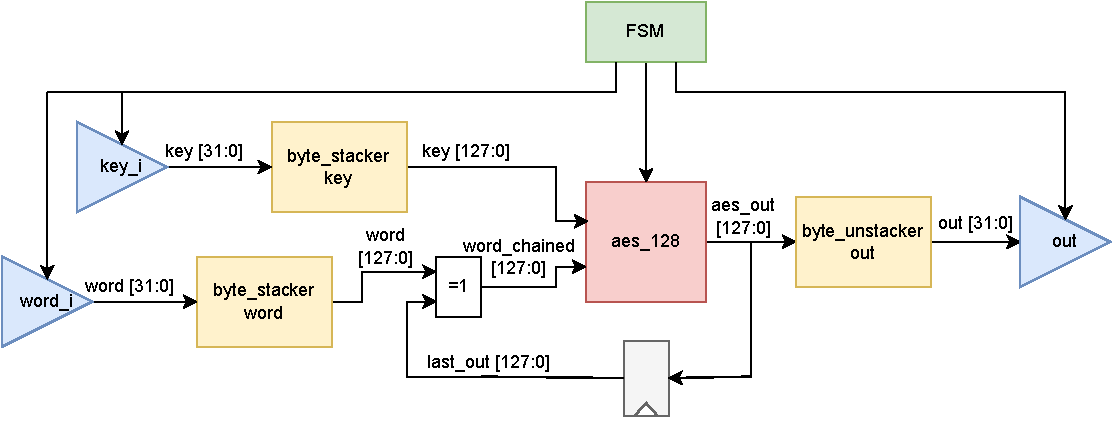
\includegraphics[width=0.95\textwidth]{hwpe_aes_update.pdf}
	\label{hwpe-aes-update}
	\caption{Block diagram of the improved AES HWPE}
\end{figure}

The used reference software implementation \cite{tiny-aes-c} already provides build-in CBC support and thus only a preprocessor flag has to be set. Again, a short self-checking demo application was written both for the PULPissimo CPU using the library and the HWPE. Both use the same set of data, to make sure the cipher feedback is done correctly, blocks of four encryptions are executed. In contrast, the ECB demo program performed only a single 128-bit encryption.

\subsection{FPGA Demonstration}

A major part of this project was evaluating the AES HWPE on an FPGA target as FPGA synthesis was not achieved during the prior course. Initially, the selected target was the Digilent Nexys~4~DDR board which is supported by the scripts in the PULPissimo repository. However, the design fills the board almost entirely (s. \Cref{sec:improvements:results}) which makes placement and routing times extremely long. Furthermore, an external JTAG debugger is required to run code on the SoC as the built-in JTAG interface is not supported. Therefore, the Digilent Genesys~2 evaluation board was selected as it features a significantly larger Xilinx FPGA from the same generation and the provided synthesis scripts support its on-board JTAG unit.

As outlined in \Cref{sec:implementation:setup}, a mounted file system was used to work both on the institute's EDA server and a local machine. This however caused problems with Vivado 2020.2 which seems to have issues when running synthesis on mounted files. Thus, a local copy of the files was made to execute FPGA synthesis. Additionally, the FPGA designs use a different top-level file than the simulation model, thus the \verb|ENABLE_HWPE| parameter has to be set again.

Executing an application with PULPissimo on an FPGA requires a debugging session consisting of a debugger (usually gdb) and an OpenOCD server providing an interface to the on-board JTAG unit. \todo{explain demo setup (clk freq)}

\subsection{Results} \label{sec:improvements:results}

\subsubsection{Performance}

Both the reference software implementation and the HPWE code were simulated and the runtimes recorded. All outputs checks passed. As the runtimes for the hardware implementation were hardly measurable from the software, they have been measured in the waveforms. \Cref{tab:results-ecb} compares the software implementation, the baseline HWPE and the slightly improved HWPE. Clearly, hardware implementations outperform the software -- which can not make use of any hardware-accelerated encryption primitives -- by factors of more than $300$. The register reduction yields a speed-up of one cycle per encryption. This somehow contradicts that two registers were removed in the datapath. However, the datapath is no standard pipeline but features ready-valid handshakes that stall some parts for a significant share of the runtime. The code size decreases for hardware implementations as the AES functionality (including relatively large look-up tables) is offloaded to hardware. Note that the code size given here is for the full demo program and thus includes not only the AES encryption but also several system routines.

\begin{table}[h]
    \centering
    \begin{tabular}{c|c c c}
        \toprule
         &  Software & HWPE (baseline) & HWPE (less registers) \\
        \midrule
		Runtime per encryption & \SI{91}{\mu s} & \SI{280}{ns} ($14$ cycles) & \SI{260}{ns} ($13$ cycles) \\
		Relative speed-up & 1 & 325 & 350 \\
		Code size [bytes] & 9824 & 9140 & 9140\\
        \bottomrule
    \end{tabular}
	\label{tab:results-ecb}
	\caption{Simulation results for different AES ECB implementations. The simulation clock frequency is \SI{50}{MHz} and the used engine was Mentor Questasim.}
\end{table}

So far, only the ECB mode was considered. \Cref{tab:results-cbc} gives runtime and code size for CBC implementations in software and hardware. Here, the encryptions take slightly longer than for ECB. The hardware has to wait for one cycle until the previous ciphertext is available, this causes one clock cycle delay. However, the speedup is still in the same order of magnitude. The larger code sizes are less related to the complexity of CBC but mainly to the larger test data used in the demo program.

\begin{table}[h]
    \centering
    \begin{tabular}{c|c c}
        \toprule
         &  Software & HWPE (CBC)  \\
        \midrule
		Runtime per encryption & \SI{91.5}{\mu s} & \SI{280}{ns} ($14$ cycles) \\
		Relative speed-up & 1 & 326.8 \\
		Code size [bytes] & 10052 & 9320 \\
        \bottomrule
    \end{tabular}
	\label{tab:results-cbc}
	\caption{Simulation results for different AES CBC implementations. The simulation clock frequency is \SI{50}{MHz} and the used engine was Mentor Questasim.}
\end{table}

\subsubsection{FPGA Resources}

Synthesis was firstly performed for the Digilent Nexys~4~DDR board. Here, the different variants of the AES HWPE yielded the resource consumptions given in \Cref{tab:results-nexys}. Clearly, removing the pipelining registers did not only improve the performance but also reduced the resource footprint notably -- mainly due to the large data width of the registers (128 bits). Cipher block chaining adds one register and an XOR block, thus its resource consumption is larger -- however it is still below the baseline ECB implementation.

\begin{table}[h]
    \centering
    \begin{tabular}{c|c c c}
        \toprule
        Resource &  HWPE (baseline) & HWPE (less registers) & HWPE (CBC)  \\
        \midrule
		Look-up-tables & 4901 & 4695 & 4819 \\
		Registers & 3780 & 3393 & 3522 \\
        \bottomrule
    \end{tabular}
	\label{tab:results-nexys}
	\caption{Resource consumption of the AES HWPE top module when synthesised for the Nexys~4~DDR evaluation board for different hardware configurations.}
\end{table}

As the final FPGA demonstration setup uses an Genesys~2 evaluation board, \Cref{tab:results-genesys} summarises the resource consumption of different entities after synthesis for this target. Clearly, there is still plenty of headroom on the board -- this simplifies placement and routing. The HWPE introduces an overhead of \SI{8.8}{\percent} for LUTs and \SI{8.3}{\percent} for registers respectively. However, the main contributor is not the datapath (HWPE engine) but the HWPE streamer which provides the interface to the tighlty-coupled data memory.

\todo{update}
\begin{table}[h]
    \centering
    \begin{tabular}{c|c c c}
        \toprule
        Entity &  Look-up-tables & Registers & BRAM tiles \\
        \midrule
		FPGA &  203800 &  407600 &  445 \\
		PULPissimo &  59574 &  45562 &  144 \\
		HWPE top &  4834 &  3522 &  0 \\
		HWPE control &  474 &  278 &  0 \\
		HWPE streamer &  2804 &  2147 &  0 \\
		HWPE engine &  1552 &  1097 &  0 \\
		AES Core &  1247 &  530 &  0 \\
		Byte stacker (each) &  25 &  131 &  0 \\
		Byte unstacker &  104 &  164 &  0 \\
        \bottomrule
    \end{tabular}
	\label{tab:results-genesys}
	\caption{Resource consumption of the PULPissimo SoC when synthesised for the Genesys~2 evaluation board.}
\end{table}

\section{ASIC Synthesis} \label{sec:asic}

As the PULP platform is mainly concerned with energy efficiency, the designs are aimed at low-power ASIC technologies (while FPGA is mainly used for prototypting). Therefore, it is interesting to perform ASIC synthesis of the AES engine to obtain comparable area and power figures.

As ASIC implementation is only briefly touched in the TU Wien Embedded Systems curriculum, a major part of the project was getting familiar with the required technologies and tools. Due to their widespread use and availability at the ICT, the Cadence toolchain and the TSMC \SI{65}{nm} technology were used. Further details are discussed in \Cref{sec:asic:tools}.

As the PULPissimo SoC has been taped out several times~\cite{pulp-chips}, the initial goal was bringing the AES HWPE to a layout. However, as discussed in \Cref{sec:asic:verification}\todo{update?}, the synthesis results were not reliably correct. As the HWPE streamer and control part (s. \Cref{hwpe-arch}) are part of several silicon-proven designs, the scope of this project was reduced to the synthesis and implementation of the new part, which is in essence the HWPE datapath depicted in \Cref{hwpe-aes-update}.

\todo{scope (including justification)}

\subsection{Technology and Tooling} \label{sec:asic:tools}

\subsection{Synthesis} \label{sec:asic:synthesis}

\subsection{Implementation} \label{sec:asic:synthesis}

\subsection{Verification} \label{sec:asic:verification}

\todo{where to place this?}
After synthesising the whole HWPE and embedding it into the PULPissimo testbench, simulation errors occur. Those are related to the control circuitry as the base address for the HWPE memory accesses is zero (instead of the address passed in the program). Likely, this issue is related to the register file in the HWPE control section which is implemented as latch. Unfortunately, no solution was found for this problem in reasonable time, thus the ASIC synthesis in this project is limited to the HWPE datapath.

\subsection{Results} \label{sec:asic:results}


\section{Summary and Outlook} \label{sec:summary}


\clearpage
\sloppy
\printbibliography

\end{document}
